\chapter{Introduction}
\label{chap:intro}
Traditionally, people rely on a single supercomputer to calculate data or deploy their companies' applications. Nowadays, cloud computing has been used widely. People would like to use a lot of normal computers and gather them into a cluster to replace a supercomputer. An increasing number of companies build their data centres or use cloud platforms to construct their business application.
However, the more computers we have, the larger of a power consumption problem we have to solve. At the same time, to make sure every computers' process in the cluster are alive, high availability becomes a more important role in cloud computing.

Virtualization is a popular technology that is used wildly in cloud computing, including virtual operating systems, computer hardware platforms, storage devices and computer network resources.
Virtual Machine is a technology to emulate a particular computer like a real computer. It can partition the physical machine's resources, such as CPU, memory, storage, and network.
A hypervisor uses execution to manage and share the host physical machine hardware, it allows many different Virtual Machines to be isolated from each other.

Container is an operating system level virtualization which runs as an isolated process in userspace on the host operating system and shares the same operation system kernel with other containers.
It provides kernel namespace such as PID, IPC, network, mount, and user namespace to isolate each container environment from the host operation system.
In order to control hardware resource such as CPU, memory, network, and disk I/O, container uses cgroups to limit each of the containers resources.
Container doesn't have hypervisor to isolate from the host operating system, therefore, it can offer better performance than Virtual Machine. There are already many software to control container, such as LXC \cite{helsley2009lxc}, LXD, Open VZ. For now, Docker \cite{Docker} is the most popular container engine. The Virtual Machine and Container architecture is shown as Fig \ref{fig:VM_vs_container}.

\begin{figure}[h]
\begin{center}
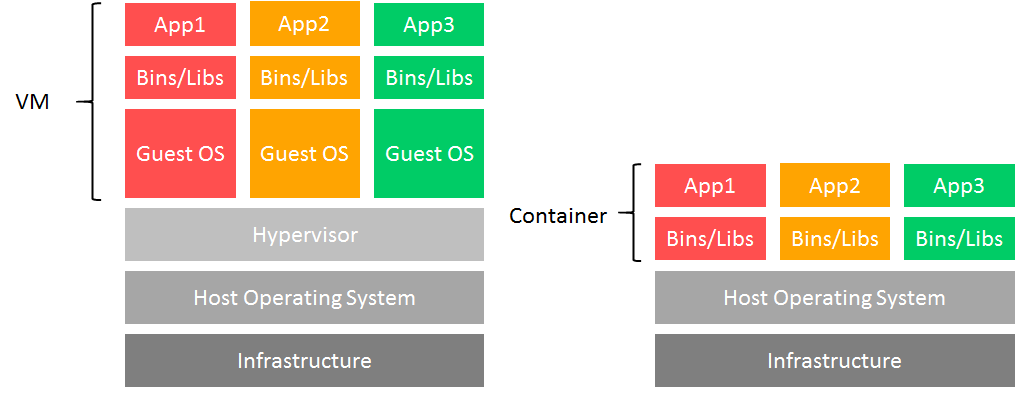
\includegraphics[width=15cm]{figure/VM_vs_container.png}
\end{center}
\caption{Virtual Machine and Container architecture}
\label{fig:VM_vs_container}
\end{figure}

Checkpoint and restoration can freeze a running process state and save process information to checkpoint images. It can be used to checkpoint image files to restore the process state. These features can be used to checkpoint and restore containers because each container is a process in the host operating system.

In this paper, we choose container but not Virtual Machine to do migration between two host machines, because container need less disk storage and less network transport resources. We not only use checkpoint and restoration to migrate the containers between two physical computers but also migrate the containers in the Docker Swarm cluster.
Moreover, we improve high availability and rescheduling feature in Docker Swarm using checkpoint and restoration than keep versions of container checkpoint images in the remote storage server that whenever the computer fails, Docker Swarm manager will restore the containers from the checkpoint images. In some cases, we use pre-dump and track-memory to save about 10\% ~ 20\% container checkpoint frozen time and at least 200\% storage space.
